\documentclass{standalone}
\usepackage{tikz}
\usepackage{ctex,siunitx}
\usepackage{tkz-euclide}
\usepackage{amsmath}
\usetikzlibrary{patterns, calc}
\usetikzlibrary {decorations.pathmorphing, decorations.pathreplacing, decorations.shapes,}
\begin{document}
\small
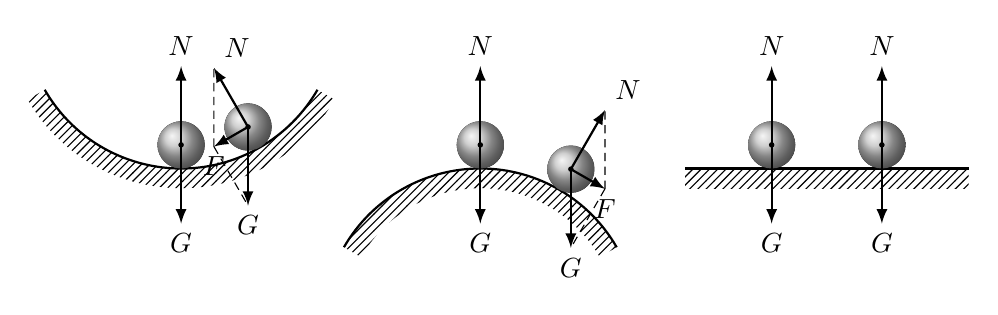
\begin{tikzpicture}[>=latex,scale=1.0]
  \fill[pattern=north east lines](210:2.0)--(210:2.25)arc(210:330:2.25)--(330:2.0)arc(330:210:2.0);
  \draw[thick](210:2.0)arc(210:330:2);
  \fill[ball color=lightgray](0,-1.7)circle(0.3);
  \fill[ball color=lightgray](-60:1.7)circle(0.3);
  \fill(0,-1.7)circle(1pt);
  \fill(-60:1.7)circle(1pt);
  \draw[thick,->](0,-1.7)--++(0,-1.0)node[below]{$G$};
  \draw[thick,->](0,-1.7)--++(0,1.0)node[above]{$N$};
  \draw[thick,->](-60:1.7)--++(0,-1.0)node[below]{$G$};
  \coordinate(F) at ([shift=(210:0.5)]-60:1.7);
  \draw[thick,->](-60:1.7)--(F)node[below]{$F$};
  \draw[thick,->](-60:1.7)--([yshift=1cm]F)node[above right]{$N$};
  \draw[thin,densely dashed](F)--++(0,1)(F)--([yshift=-1cm]-60:1.7);
  \begin{scope}[xshift=3.8cm,yshift=-4cm]
    \fill[pattern=north east lines](150:2.0)--(150:1.75)arc(150:30:1.75)--(30:2.0)arc(30:150:2.0);
    \draw[thick](150:2.0)arc(150:30:2);
    \fill[ball color=lightgray](0,2.3)circle(0.3);
    \fill[ball color=lightgray](60:2.3)circle(0.3);
    \fill(0,2.3)circle(1pt);
    \fill(60:2.3)circle(1pt);
    \draw[thick,->](0,2.3)--++(0,-1.0)node[below]{$G$};
    \draw[thick,->](0,2.3)--++(0,1.0)node[above]{$N$};
    \draw[thick,->](60:2.3)--++(0,-1.0)node[below]{$G$};
    \coordinate(F') at ([shift=(-30:0.5)]60:2.3);
    \draw[thick,->](60:2.3)--(F')node[below]{$F$};
    \draw[thick,->](60:2.3)--([yshift=1cm]F')node[above right]{$N$};
    \draw[thin,densely dashed](F')--++(0,1)(F')--([yshift=-1cm]60:2.3);
  \end{scope}
  \begin{scope}[xshift=8.2cm,yshift=-2cm]
    \fill[pattern=north east lines](-1.8,0)rectangle(1.8,-0.25);
    \draw[thick](-1.8,0)--(1.8,0);
    \foreach \x in {0.7,-0.7}
    {
      \fill[ball color=lightgray](\x,0.3)circle(0.3);
      \fill(\x,0.3)circle(1pt);
      \draw[thick,->](\x,0.3)--++(0,-1.0)node[below]{$G$};
      \draw[thick,->](\x,0.3)--++(0,1.0)node[above]{$N$};
    }
  \end{scope}
\end{tikzpicture}
\end{document}